% !TEX encoding = UTF-8 Unicode
\documentclass{article}

\usepackage{polski}
\usepackage[utf8]{inputenc}
\usepackage{subfig}
\usepackage{multirow}
\usepackage{graphicx}

\usepackage[a4paper, left=2.5cm, right=2.5cm, top=3.5cm, bottom=3.5cm, headsep=1.2cm]{geometry}

\linespread{1.3}
\begin{document}
	
	\begin{titlepage}
		\centering
		{\scshape\LARGE Politechnika Wrocławska \par}
		{\scshape\Large Katedra Informatyki Technicznej\par}
		
		\vspace{1cm}
		{\scshape\Large Inżynieria Oprogramowania\par}
		\vspace{1.5cm}
		{\huge\bfseries \par}
		\vspace{2cm}
		{\Large\itshape Magdalena Biernat\par}
		{\Large\itshape Mateusz Bortkiewicz\par}
		\vfill
		Opiekun\par
		prof. dr hab. inż. Jan Magott 
		
		\vfill
		{\large \today\par}
	\end{titlepage}
	\newpage
	
	\section{Wprowadzenie}
	Sprawozdanie dotyczy ósmych zajęć. Na tych laboratoriach kontynuowaliśmy swój projekt. 
	
	\subsection{Cel laboratorium}
Definiowanie w sposób iteracyjno - rozwojowy modelu projektowego
programowania opartego na:
\begin{itemize}
\item Modelowaniu logiki biznesowej reprezentowanej przez wybrany
bazowy przypadek użycia za pomocą diagramów sekwencji, gdzie
diagram klas pełni rolę struktury komunikacji wykorzystanej podczas
tworzenia diagramów sekwencji. Ten model i implementacja przypadku
użycia powinien stanowić bazę operacji stosowanych w kolejnych
iteracjach. Należy definiować operacje i atrybuty kolejnej klasy
(dziedziczenie, powiązania i agregacje) na diagramie klas
zidentyfikowanej w wyniku modelowania kolejnego przypadku użycia i
wykonanie scenariusza tego przypadku użycia za pomocą diagramu
sekwencji.
\item Implementacja modelu projektowego wybranego przypadku użycia za
pomocą języka Java SE.
\end{itemize}
	\subsection{Plan pracy}
	Zadania wykonaliśmy wg instrukcji 6:
	
	\begin{itemize}
		\item Diagram sekwencji wypożyczenia
		\item Diagram sekwencji szukania wypożyczenia
	\end{itemize}
	\newpage
	\section{Laboratorium}
	\subsection{ Diagram sekwencji wypożyczenia}
\begin{figure}[!ht]
	\centering
	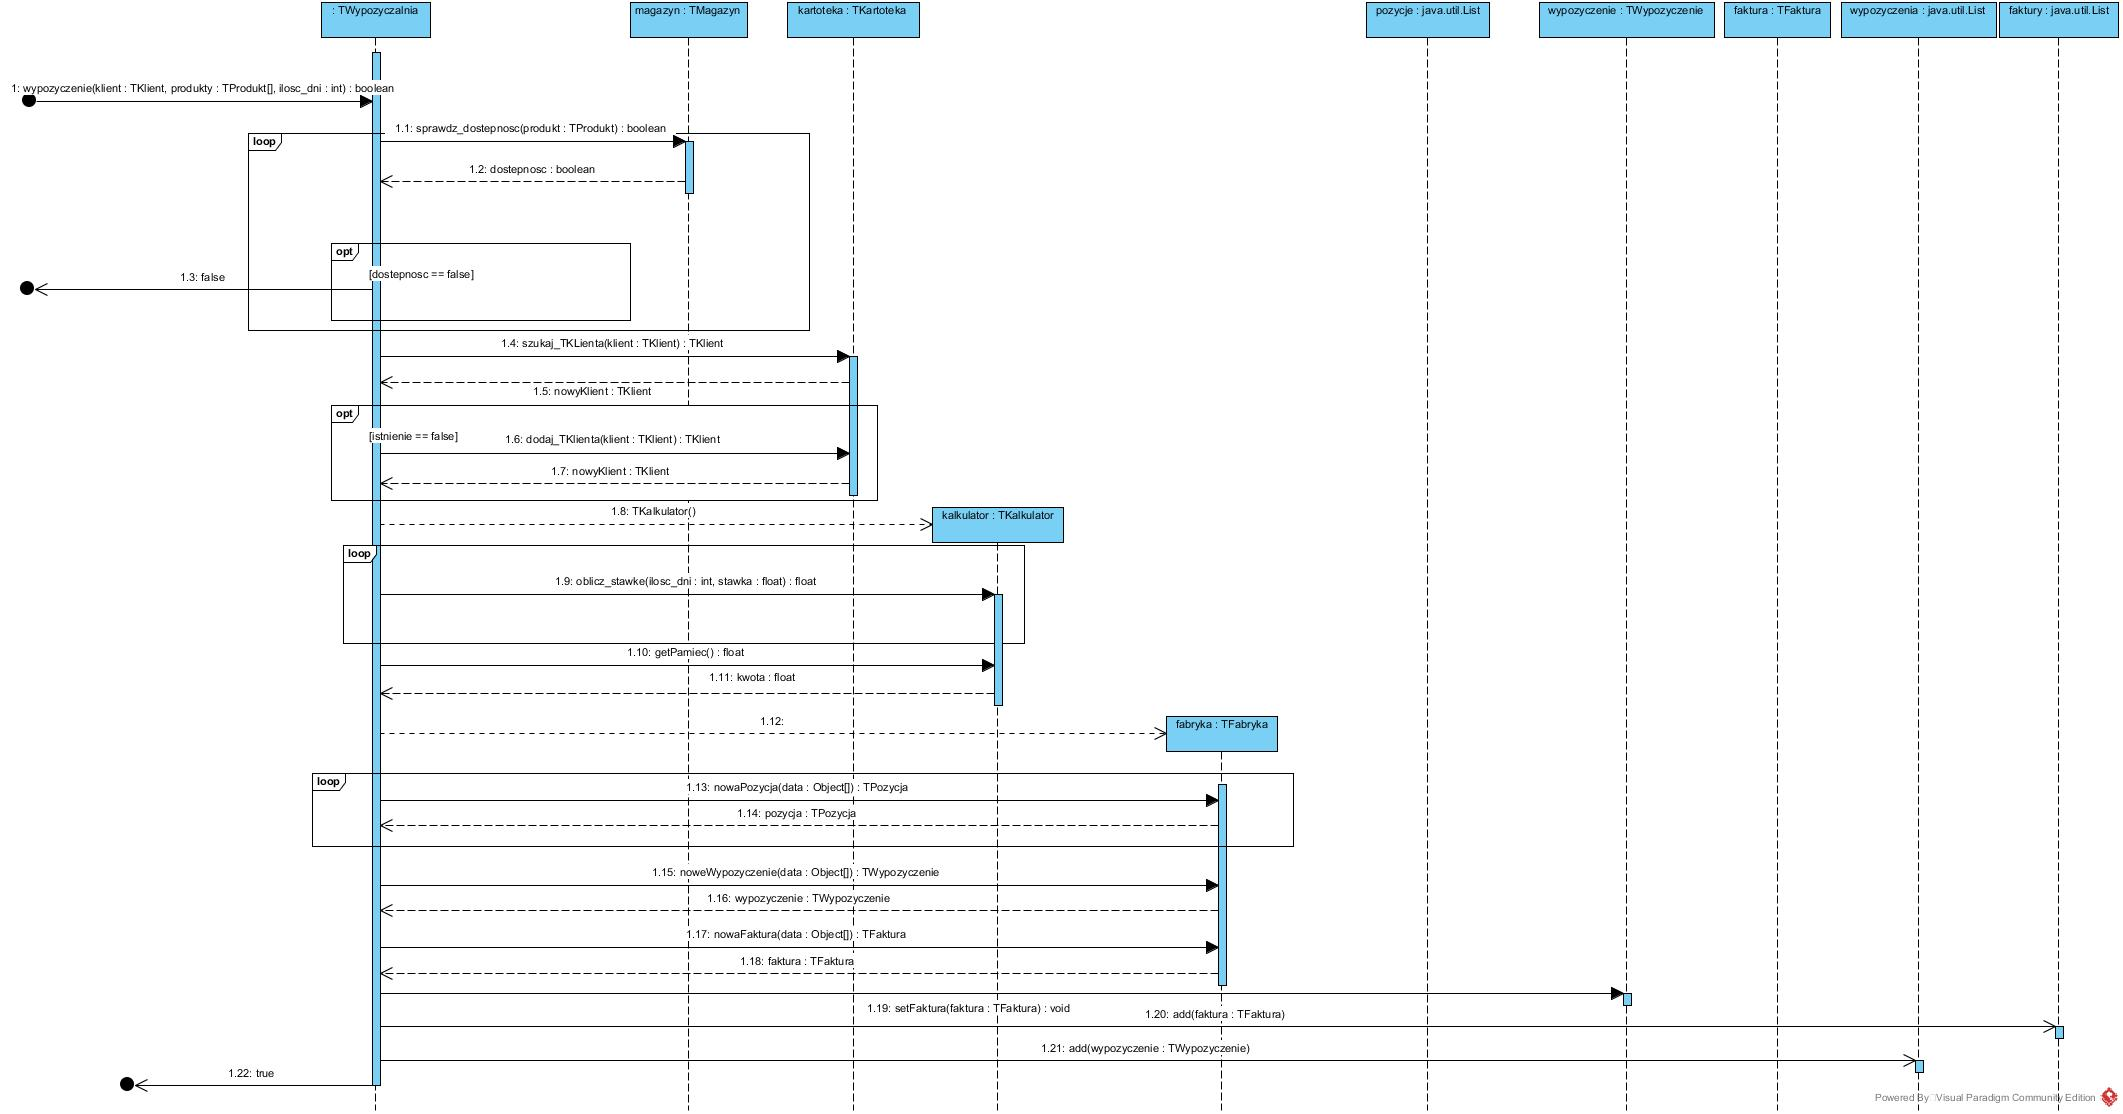
\includegraphics[angle=270,width=10cm]{Diagram_sekwencji_wypozyczenia_nowy.jpg}
	\caption{Stworzony diagram sekwencji}
	\label{fig:obrazek 1}
\end{figure}
	\newpage
	\subsection{Diagram sekwencji szukania wypożyczenia }
	\begin{figure}[!ht]
	\centering
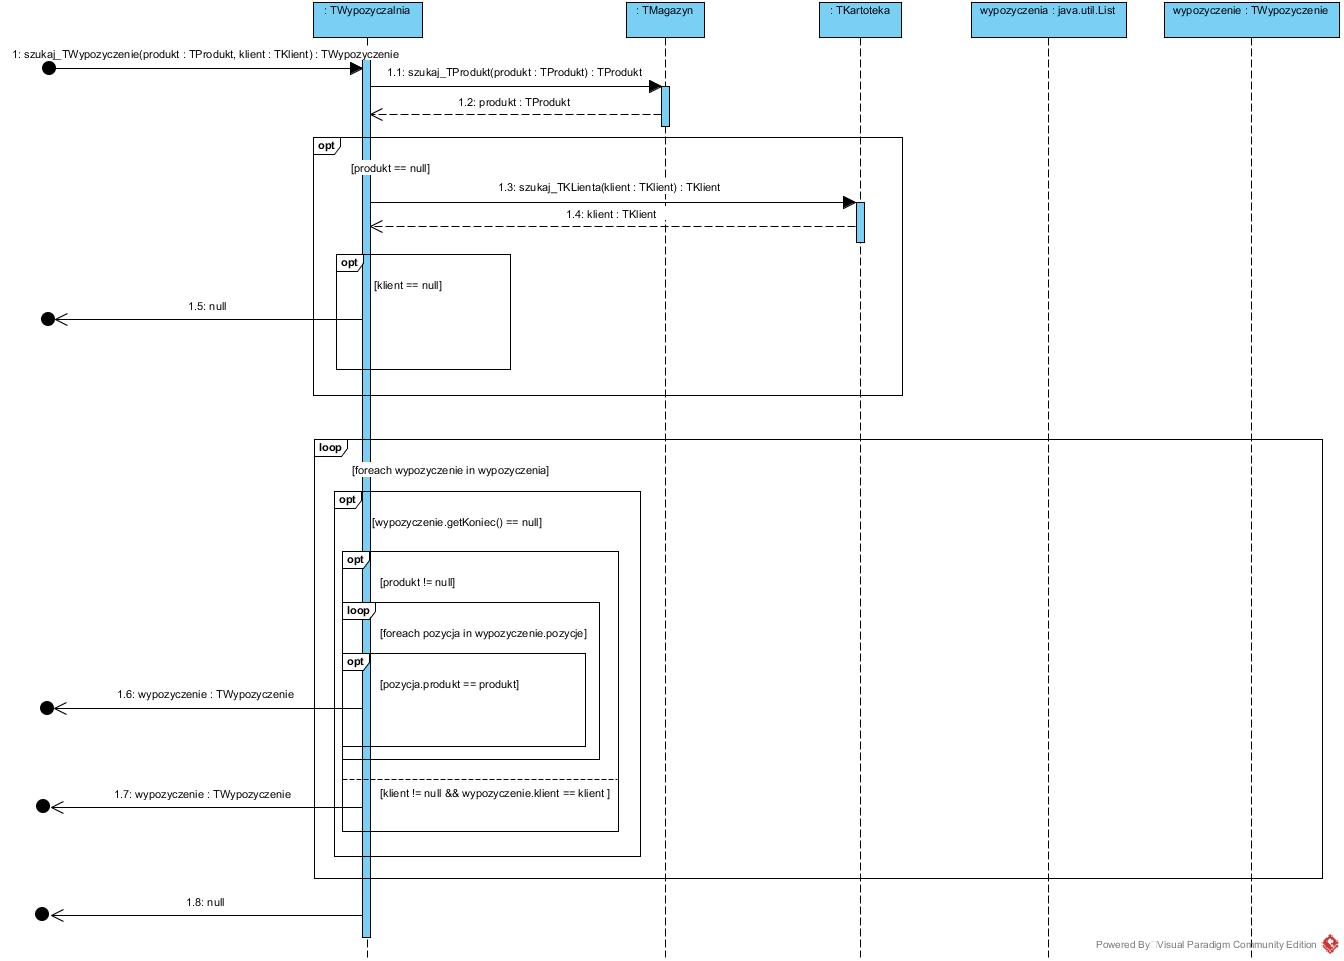
\includegraphics[angle=270,width=14cm]{Diagram_sekwencji_szukanie_wypozyczenia.jpg}
\caption{Stworzony diagram sekwencji}
\label{fig:obrazek 2}
	\end{figure}
\subsection{Diagram klas}
Diagram klas sukcesywnie zostaje uzupełniany o kolejne elementy.
	\begin{figure}[!ht]
	\centering
	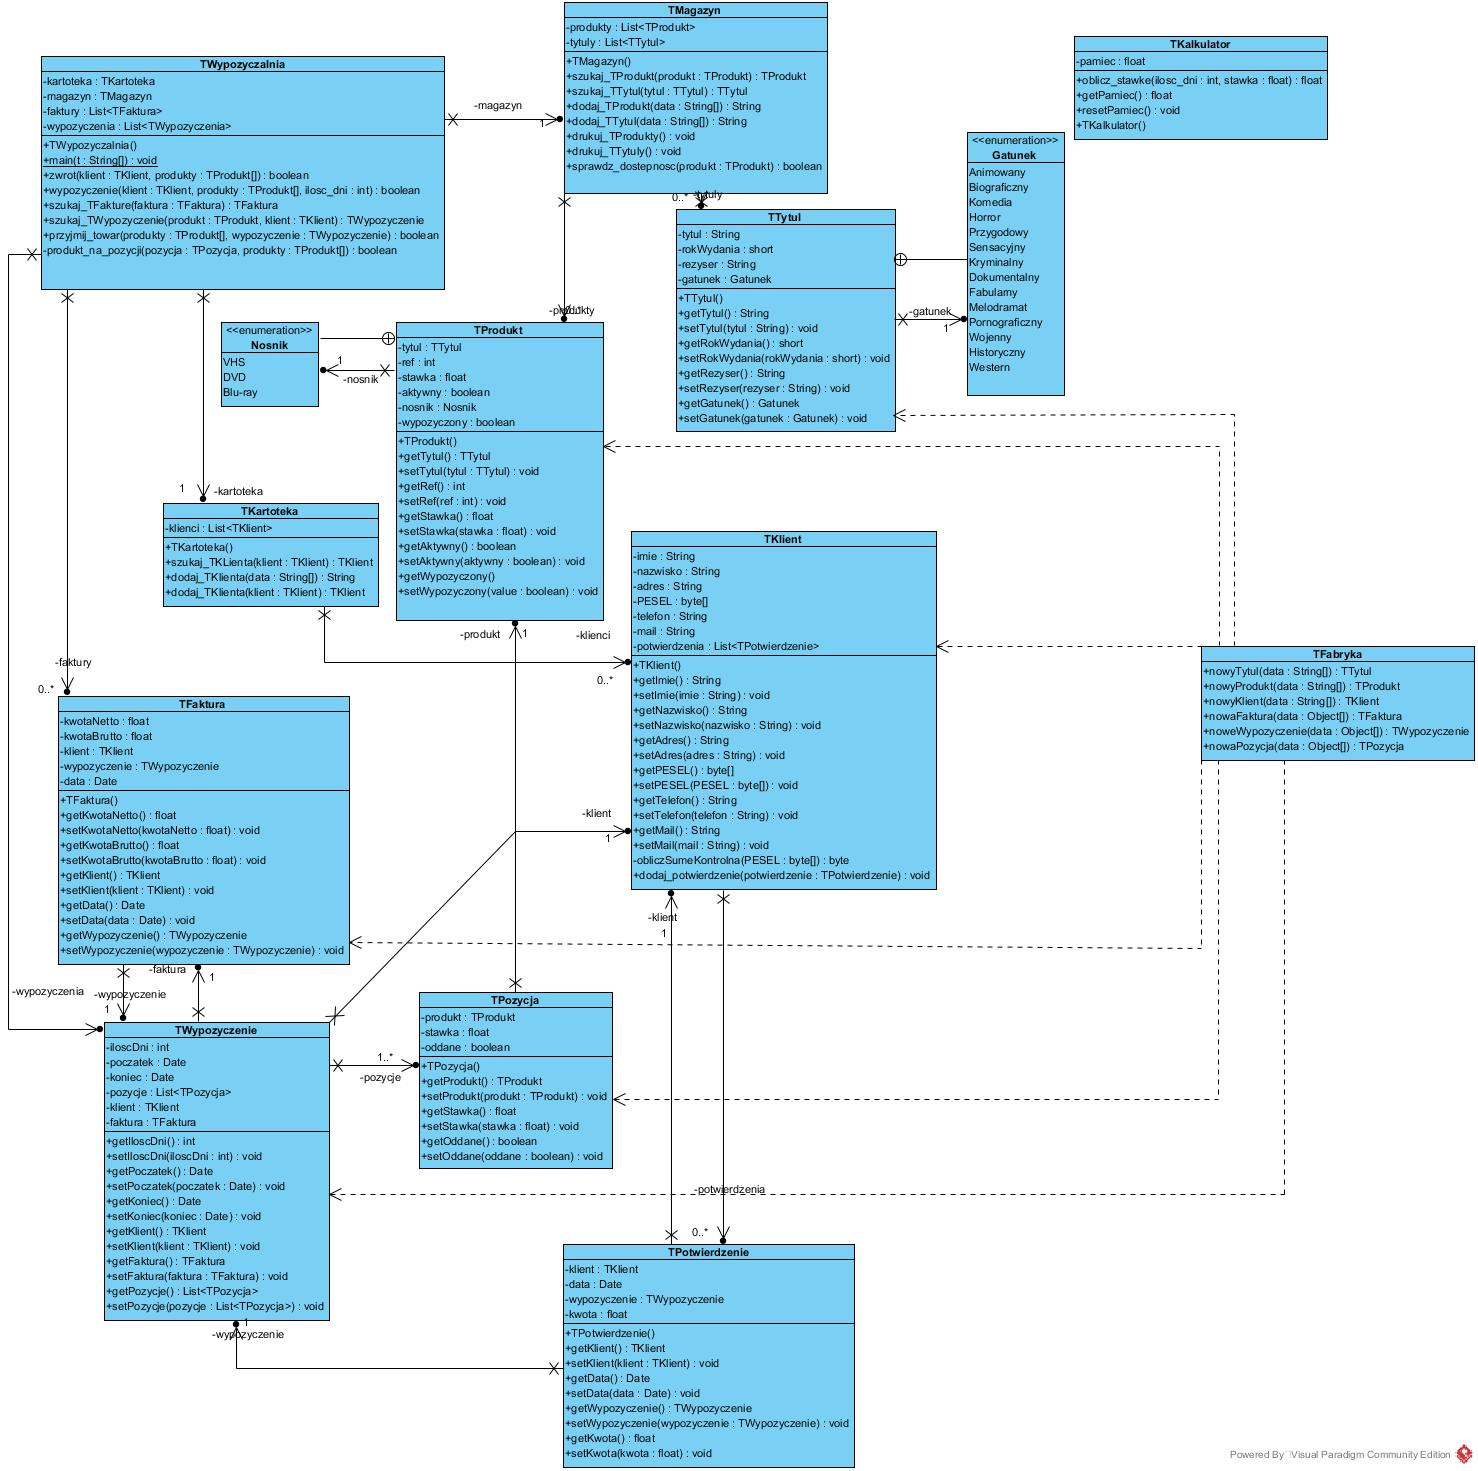
\includegraphics[width=17.5cm]{Diagram_klas.jpg}
	\caption{Stworzony diagram klas}
	\label{fig:obrazek 3}
\end{figure}
\end{document}